\section{Information extraction}

\subsection{Populating knowledge bases}
Manual creation of knowledge bases is expensive: automate it?
Extract knowledge from documents but knowledge is encoded in natural
language. \\
Intended results
\begin{itemize}
\item Automated or accelerated creation of knowledge bases
\item Support for structured search on documents
\end{itemize}

\subsection{Concepts and statements}
Concepts are \textbf{ideas} or concrete \textbf{entities} that are
explicitly mentioned in a document.
\begin{itemize}
\item expresses as words or phrases in natural language
\item different to topics, they are implicit mentions of ideas
\item representation of concepts can be directly understood and
  interpreted by humans
\item concepts can have relationships: \textbf{statements}
\end{itemize}

\subsection{Identifying concepts in documents}
Sometimes they are supplied explicitly by authors
\begin{itemize}
\item hashtags in tweets
\item keywords in scientific articles
\end{itemize}
Most of the time, need to be extracted

\subsection{Keyphrase extraction}
Automatic selection of important and topical phrases from the body of
a document.
\begin{itemize}
\item document summarization, search and indexing
\item document classification and opinion mining
\end{itemize}

aims at identify words and phrases typical for the document.

\subsection{Keyphrase extraction methods}
generate candidate phrases and rank them
\begin{itemize}
\item remove stopwords
\item use word n-grams
\item select based on PoS tags
\end{itemize}

Baseline ranking approach
\begin{itemize}
\item rank candidate phrase of the document according to their tf-idf
  value
\end{itemize}
more advanced
\begin{itemize}
\item use of many structural, syntactic features of the document
\item use of external resources, wikipedia, wordnet\ldots
\end{itemize}

\subsection{Uses of keyphrase extraction}
\begin{itemize}
\item Creation of domain-specific thesaurus and taxonomy
\item Document classification and search
\end{itemize}

\subsection{Named entity recognition}
\textbf{Task}: Find and classify names of peoples, organisations,
places, brands, etc.\ that are mentioned in documents

\subsection{Uses of NER}
\begin{itemize}
\item Named entities can be indexed, linked, etc.\
\item Sentiment can be attributed to companies or products
\item Information extraction can use named entities as anchor
\end{itemize}

\subsection{NER as sequence labelling task}
Sequence of tags, indicating whether the word is inside (I) or outside
(O) an entity. Classification problem!

When an entity name is dtected it can be classified to the type of the
entity, e.g.\ an organisation (ORG), a location (GEO), a person, etc.\

\subsection{NER as classification task}
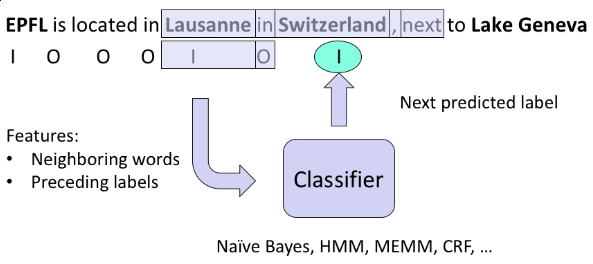
\includegraphics[width=200px, height=120px]{ner}

\subsection{Features used in NER}
\textbf{EPFL} is located in \textbf{Lausanne} in \textbf{Switzerland},
next to \textbf{Lake Leman}. \\
Features of ``Lausanne'':
\begin{itemize}
\item Word and neighboring words: Lausanne, in
\item Part-Of-Speech tags (POS): POS(Lausanne) = NN
\item Prefixes and suffixes: prefix(Lausanne, 3) = Lau
\item Word shape: WS(Lausanne): Xxxxxxx
\item Short word shape: SWS(Lausanne) = Xx
\end{itemize}

\subsection{Generative probabilistic model}
Sequence of words(known): $ W = (w_1, w_2, \ldots, w_n) $ \\
Sequence of state (unknown): $ E = (e_1, e_2, \ldots, e_n) $ \\
Assume the text is produced by a probabilistic process: $ P(E, W) $

Find the most probable model $ argmax_E P(E \mid W) $ \\
Bayes Law: $ argmax_E P(E \mid W) = argmax_E P(E)P(W \mid E) $

\subsubsection{Approximation}
Label transition probabilities (bigram model) \\
$ P(E) = P(e_1, \ldots, e_n) \approx \prod_{i = 2, \ldots, n} P_E(e_i
\mid e_{i - 1}) $ \\

Word emission probabilities: \\
$ P(W \mid E) = \prod_{i = 1, \ldots, n} P_W(w_i \mid e_i) $

Since it is not possible to estimate the complet probability
distribution we approximate by making independence assumptions. We
assume that the probability of a label to occur depends only on the
previous label.

\subsection{Hidden Markov Model}
Assume the text is produced by a probabilistic process (with unknown
transition probabilities)

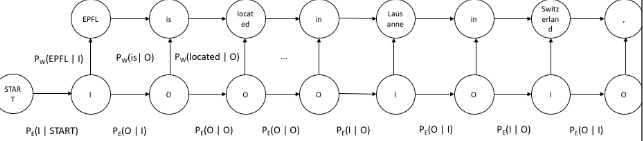
\includegraphics[width=200px, height=40px]{hmm}
Maximum likelihood estimation, e.g.\ \\
$ P_E(I \mid O) = \frac{2}{5} $, $ P_w(in \mid O) = \frac{2}{5} $

We can represent approximate model of the probability distribution as
a Markov Model, where we indicate which probabilistic variables depend
on which others.

We use maximum likelihood estimation for estimating $ P_E(e_i \mid
e_{i - 1})$ and $ P_W(w_i \mid e_i) $.

\subsection{Smoothing}
Unseen words might only miss in the training set: \\
$ P_{WS} (w_i \mid e_) = \lambda P_W(w_i \mid e_i) + (1- \lambda)
\frac{1}{n} $

For labels no smoothing needed, all labels occur in the training set.

\subsection{Statement extraction}
EPFL is one of the two Swiss federal institute of Technology\\
EPFL - IS-A - Swiss Federal Institute of Technology \\

its sister institution in Zurich, ETHZ \\
EPFL - RELATED-TO - ETHZ\\

Observations
\begin{itemize}
\item statements are anchored in two entities (relationship)
\item relationships can carry different meaning
\item extraction of statement can be ambiguous
\end{itemize}

\subsection{Typed statements}
EPFL - PART-OF - Swiss Federal Institute of Technology \\
Type : ORG - PART-OF - ORG \\

\subsection{Hand-written patterns}
Patterns to detecte IS-a relationships
\begin{itemize}
\item ``Y such as X ((, X)* (, and $ \mid $ or X))''
\item ``such Y as X'' \ldots
\end{itemize}

\subsubsection{Web isa database}
Example of large-scale effort to extract IS-A relationshups from Web
data.

\subsubsection{More general hand-written patterns}
Relations often hold between specific entity
\begin{itemize}
\item locate-in(ORGANIZATION, LOCATION)
\item found(PERSON, ORGANIZATION)
\item cures(DRUG, DISEASE)
\end{itemize}

First perform Named Entity Recognition

\subsubsection{Hand-writtent patterns summary}
Advantages
\begin{itemize}
\item Rules tend to be high precision
\item Can be tailored to specific domains
\end{itemize}
Disadvantages
\begin{itemize}
\item Human pattenrs are often low-recall
\item A lot of effort to think of all possible patterns
\end{itemize}

\subsection{Supervised learning for IE}
Train a classifier on labeled data. \\
Creating a training set
\begin{itemize}
\item Choose relevant named entites and their relations
\item Hand label relations among entities
\end{itemize}

\subsubsection{Classifiers for IE}
\begin{itemize}
\item A \textbf{filtering classifier}, to detect whether a relation
  exists among the entities
\item A \textbf{relation-specific classifier} detected the relation
  label
\end{itemize}

Training the classifiers
\begin{itemize}
\item Extract named entities in the document corpus using NER
\item Detect pairs of entities, e.g.\, in the same sentence
\item Use unlabeled entity pairs as negative examples
\end{itemize}

\subsubsection{Features used in IE}

Features for mention(M1, M2) = (Lausanne, Lake Leman)
\begin{itemize}
\item Bag of words (BOW) and bigrams: located in, next to, Lausanne,
  in
\item BOW and bigrams in between the mention: in, next to
\item Headwords, their concatenation: EPFL, Genevea, EPFL-Geneva
\item Words in positions: M1 + 1:is, M2-1: to
\item Stemmed version of the words
\item Types of entities: ORG, LOC, ORG-LOC
\item Syntactic features
\end{itemize}

\subsubsection{Syntactic features}
Parse tree: NLP-like! \\
Features: \\
Sequence between entitites: VP VP PP NP PP NP PP

\subsection{Bootstrapping}

No training data, but a few high-precision patterns

\begin{itemize}
\item Find entity pairs that match the pattern
\item Find sentences containing those entity pairs
\item Generalize the entities in those sentences
\item Generate new patterns
\end{itemize}

The idea is that phrases containing the entity pairs expresses the
same type of relationship in a different syntactic relationship. Thus
those sentences can be considered as templates for expressing the
relationship. And we can come up with new patterns

Example:
\begin{itemize}
\item Pattern: LOC is located in LOC
\item Mumbai is located in India
\item Search for entity pairs (Mumbai, India)
\item Mumbai is India's top destiation
\item New patterns:
\item LOC is LOC's top destination
\end{itemize}

\subsection{Semantic drift}
The pattern LOC hotels, LOC matches also \ldots Geneva hotels,
Lausanne hotels $ \rightarrow $ Geneva is located in Lausanne?

\subsubsection{Confidence}
Assume we have a confirmed set of pairs of mentions M
\begin{itemize}
\item $ Hits_p $ = set of tuples in M that a new pattern matches
\item $ Finds_p $ = total set of tuples that a new pattern matches
\end{itemize}

Confidence that a new pattern finds many relevant mentions: \\
$ Conf(p) = \frac{Hits_p}{Finds_p} log(Finds_p) $

If a pattern matches too many pairs without creating confirmed entity
pairs the confidence in the template is lowered.

\subsection{Distant supervision}

Use a large corpus of data to collect training data from which a
classifier can be trained
\begin{itemize}
\item Combines advantages of bootstraping with supervised learning
\end{itemize}

\begin{itemize}
\item Run NER on wikipedia and extract all entity pairs in sentences
  (s, ent1, ent2)
\item Check whether a relation among the entities exists in WikiData
  DB
\item For entities with relations extract features from the sentence
\item Training data = (ent2, ent2, rel, features)
\item Train a classifier to predict the relation.
\item Predit label for new sentences (s, ent1, ent2, ref?)
\end{itemize}

\subsubsection{Features for distant supervision}
Use conjuctions of standard IE features as sentence features
\begin{itemize}
\item Match only if all individual features match
\item High precision but low recall features
\item Feasible since training set is large
\end{itemize}

Complex features resemble templates used in rule-based
approaches. Instead of producing a feature vector from combining all
individual features, each feature combination is considered as a
separate feature; which result in much larger feature space. Those
more complex features are much more precise but have low
recall. Compensated by the fact that the training set is much larger.

\subsection{Summary}
\begin{itemize}
\item Populating knowledge bases and fact databases
\item Taxonomy induction
\end{itemize}
Pattern-based approaches
\begin{itemize}
\item High precision, low recall, work intensive
\end{itemize}
Supervised learning
\begin{itemize}
\item Low precision, high recall, work intensive
\end{itemize}

Hybrids methods: bootstraping, distant supervision \\
No relation schema known: open information extraction

%%% Local Variables:
%%% mode: latex
%%% TeX-master: "master"
%%% End:
